\let\negmedspace\undefined
\let\negthickspace\undefined
\documentclass[journal]{IEEEtran}
\usepackage[a5paper, margin=10mm, onecolumn]{geometry}
%\usepackage{lmodern} % Ensure lmodern is loaded for pdflatex
\usepackage{tfrupee} % Include tfrupee package

\setlength{\headheight}{1cm} % Set the height of the header box
\setlength{\headsep}{0mm}     % Set the distance between the header box and the top of the text

\usepackage{gvv-book}
\usepackage{gvv}
\usepackage{cite}
\usepackage{amsmath,amssymb,amsfonts,amsthm}
\usepackage{algorithmic}
\usepackage{graphicx}
\usepackage{textcomp}
\usepackage{xcolor}
\usepackage{txfonts}
\usepackage{listings}
\usepackage{enumitem}
\usepackage{mathtools}
\usepackage{gensymb}
\usepackage{comment}
\usepackage[breaklinks=true]{hyperref}
\usepackage{tkz-euclide} 
\usepackage{listings}
% \usepackage{gvv}                                        
\def\inputGnumericTable{}                                 
\usepackage[latin1]{inputenc}                                
\usepackage{color}                                            
\usepackage{array}                                            
\usepackage{longtable}                                       
\usepackage{calc}                                             
\usepackage{multirow}                                         
\usepackage{hhline}                                           
\usepackage{ifthen}                                           
\usepackage{lscape}
\begin{document}

\bibliographystyle{IEEEtran}
\vspace{3cm}

\title{NCERT-9.5.13}
\author{EE24BTECH11065 - Spoorthi yellamanchali
}
% \maketitle
% \newpage
% \bigskip
{\let\newpage\relax\maketitle}

\renewcommand{\thefigure}{\theenumi}
\renewcommand{\thetable}{\theenumi}
\setlength{\intextsep}{10pt} % Space between text and floats


\numberwithin{equation}{enumi}
\numberwithin{figure}{enumi}
\renewcommand{\thetable}{\theenumi}


\textbf{Question:}
\\
The difference between two numbers is 26 and one number is three times the other. Find them.
\\
\textbf{ Theoretical Solution: }
\\
Let the two numbers be $x$ and $y$ respectively,
Then, by the question, we get the equation,
\begin{align} 
x - y = 26\\
x = 3y
\end{align}
On substituting equation $\brak{0.2}$ in equation $\brak{0.1}$, we get,
\begin{align}
    3y - y = 26\\
    y = 13
\end{align}
Then,
\begin{align}
    x = 3\brak{13} = 39.
\end{align}
$\therefore$ we get, $x = 13$ and $y = 39$
\\
\textbf{Solution by LU decomposition.}
\\
Given a matrix $A$ of size $n\times n$,$LU$ decomposition is performed row by row ,column by column.
We start ny initializing $L$ as identity matrix of same order $L = I_n$,and $U$ as $A$.\\
The update equations are as follows,\\
For each column $j \geq k$, the entries of $U$ in the $k$th row are updated as:
\begin{align}
    U_{k,j} = A_{k,j} - \sum_{m=1}^{k-1} L_{k,m}.U_{m,j},   \forall{j \geq k}
\end{align}
For each row $i > k$, the entries of $L$ in the $k$th column are updated as:
\begin{align}
    L_{j,k} = \frac{1}{U_{k,k}}\brak{A_{j,k} - \sum_{m=1}^{k-1}.U_{m,k}}, \forall{i>k}
\end{align}
 given equations:
 \begin{align}
     x - y = 26\\
     x - 3y = 0
 \end{align}
 we can represent these set of equations as
 \begin{align}
     A\Bar{x} = b
 \end{align}
 where,
 \begin{align}
     A = \begin{bmatrix}
         1 & -1\\
         1 & -3
     \end{bmatrix} \\
     \Bar{x} = \begin{bmatrix}
         x\\
         y
     \end{bmatrix} \\
     b = \begin{bmatrix}
         26\\
         0
     \end{bmatrix}
 \end{align}
 Using guassian elimination algorithm,we can decompose matix $A$ into product of lower traingular matrix ($L$) and upper triangular matrix ($U$).
 \begin{align}
     A = LU.
 \end{align}
 let us first initialize
 \begin{align}
     L = \begin{bmatrix}
         1&0\\
         0&1
     \end{bmatrix}
 \end{align}
 and 
 \begin{align}
     U = A
 \end{align}
 Then on applying guassian elimination algorithm,\\
 On elminating the element (making it zero) of position (2,1) by row operations, we get,
 \begin{align}
     R_2 = R_2 - 1.R_1.
 \end{align}
 updated U becomes,
\begin{align}
    \begin{bmatrix}
        1&-1\\
        0&-2
    \end{bmatrix}
\end{align}
here , '1' is the multiplier we used.
So , on updating the position (2,1) in the matrix $L$ with the multiplier, we get the required matrices $L$ and $U$ respectively.
\begin{align}
    \therefore L = \begin{bmatrix}
        1&0\\
        1&1
    \end{bmatrix}
\end{align}
Now,equation $\brak{0.14}$ can be written as,
\begin{align}
    LU\Bar{x} = b
\end{align}
Let,
\begin{align}
    U\Bar{x} = y
\end{align}
Then,
\begin{align}
    Ly = b
\end{align}
On solving using forward substitution, we get , 
\begin{align}
    y = \begin{bmatrix}
        26\\
        -26
    \end{bmatrix}
\end{align}
Now, from equation $\brak{0.21}$, on solving for $\Bar{x}$ using backward substitution, we get,
\begin{align}
    \Bar{x} = \begin{bmatrix}
        39\\
        13
    \end{bmatrix}
\end{align}
$\therefore$ we get,
\begin{align}
    x = 39\\
    y = 13
\end{align}

\begin{figure}[h!]
   \centering
   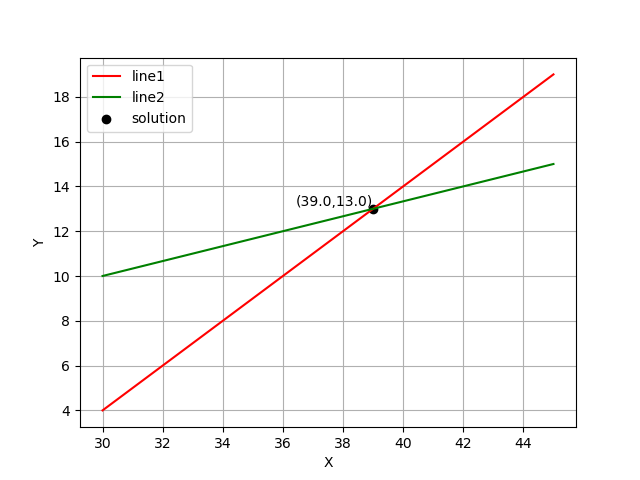
\includegraphics[width=0.75\columnwidth]{figs/Figure_1.png}
\end{figure}
\end{document}


